\documentclass[aspectratio=169]{beamer}

%\usepackage[faculty=apps,titlelogo=none,slidelogo=none]{ULiege-trigon}

% Document metadata
\subtitle{\vspace{-3em}Quantifying Integration Costs of Variable Renewable Energy Technologies in European Energy Systems}
\author{Muhammad Umair Tareen, Sylvain Quoilin}
\institute{University of Liège}
\date{ECOS, Paris - June 30, 2025}

% Image for the title page (use includegraphics option to properly size/place it)
\titlegraphic{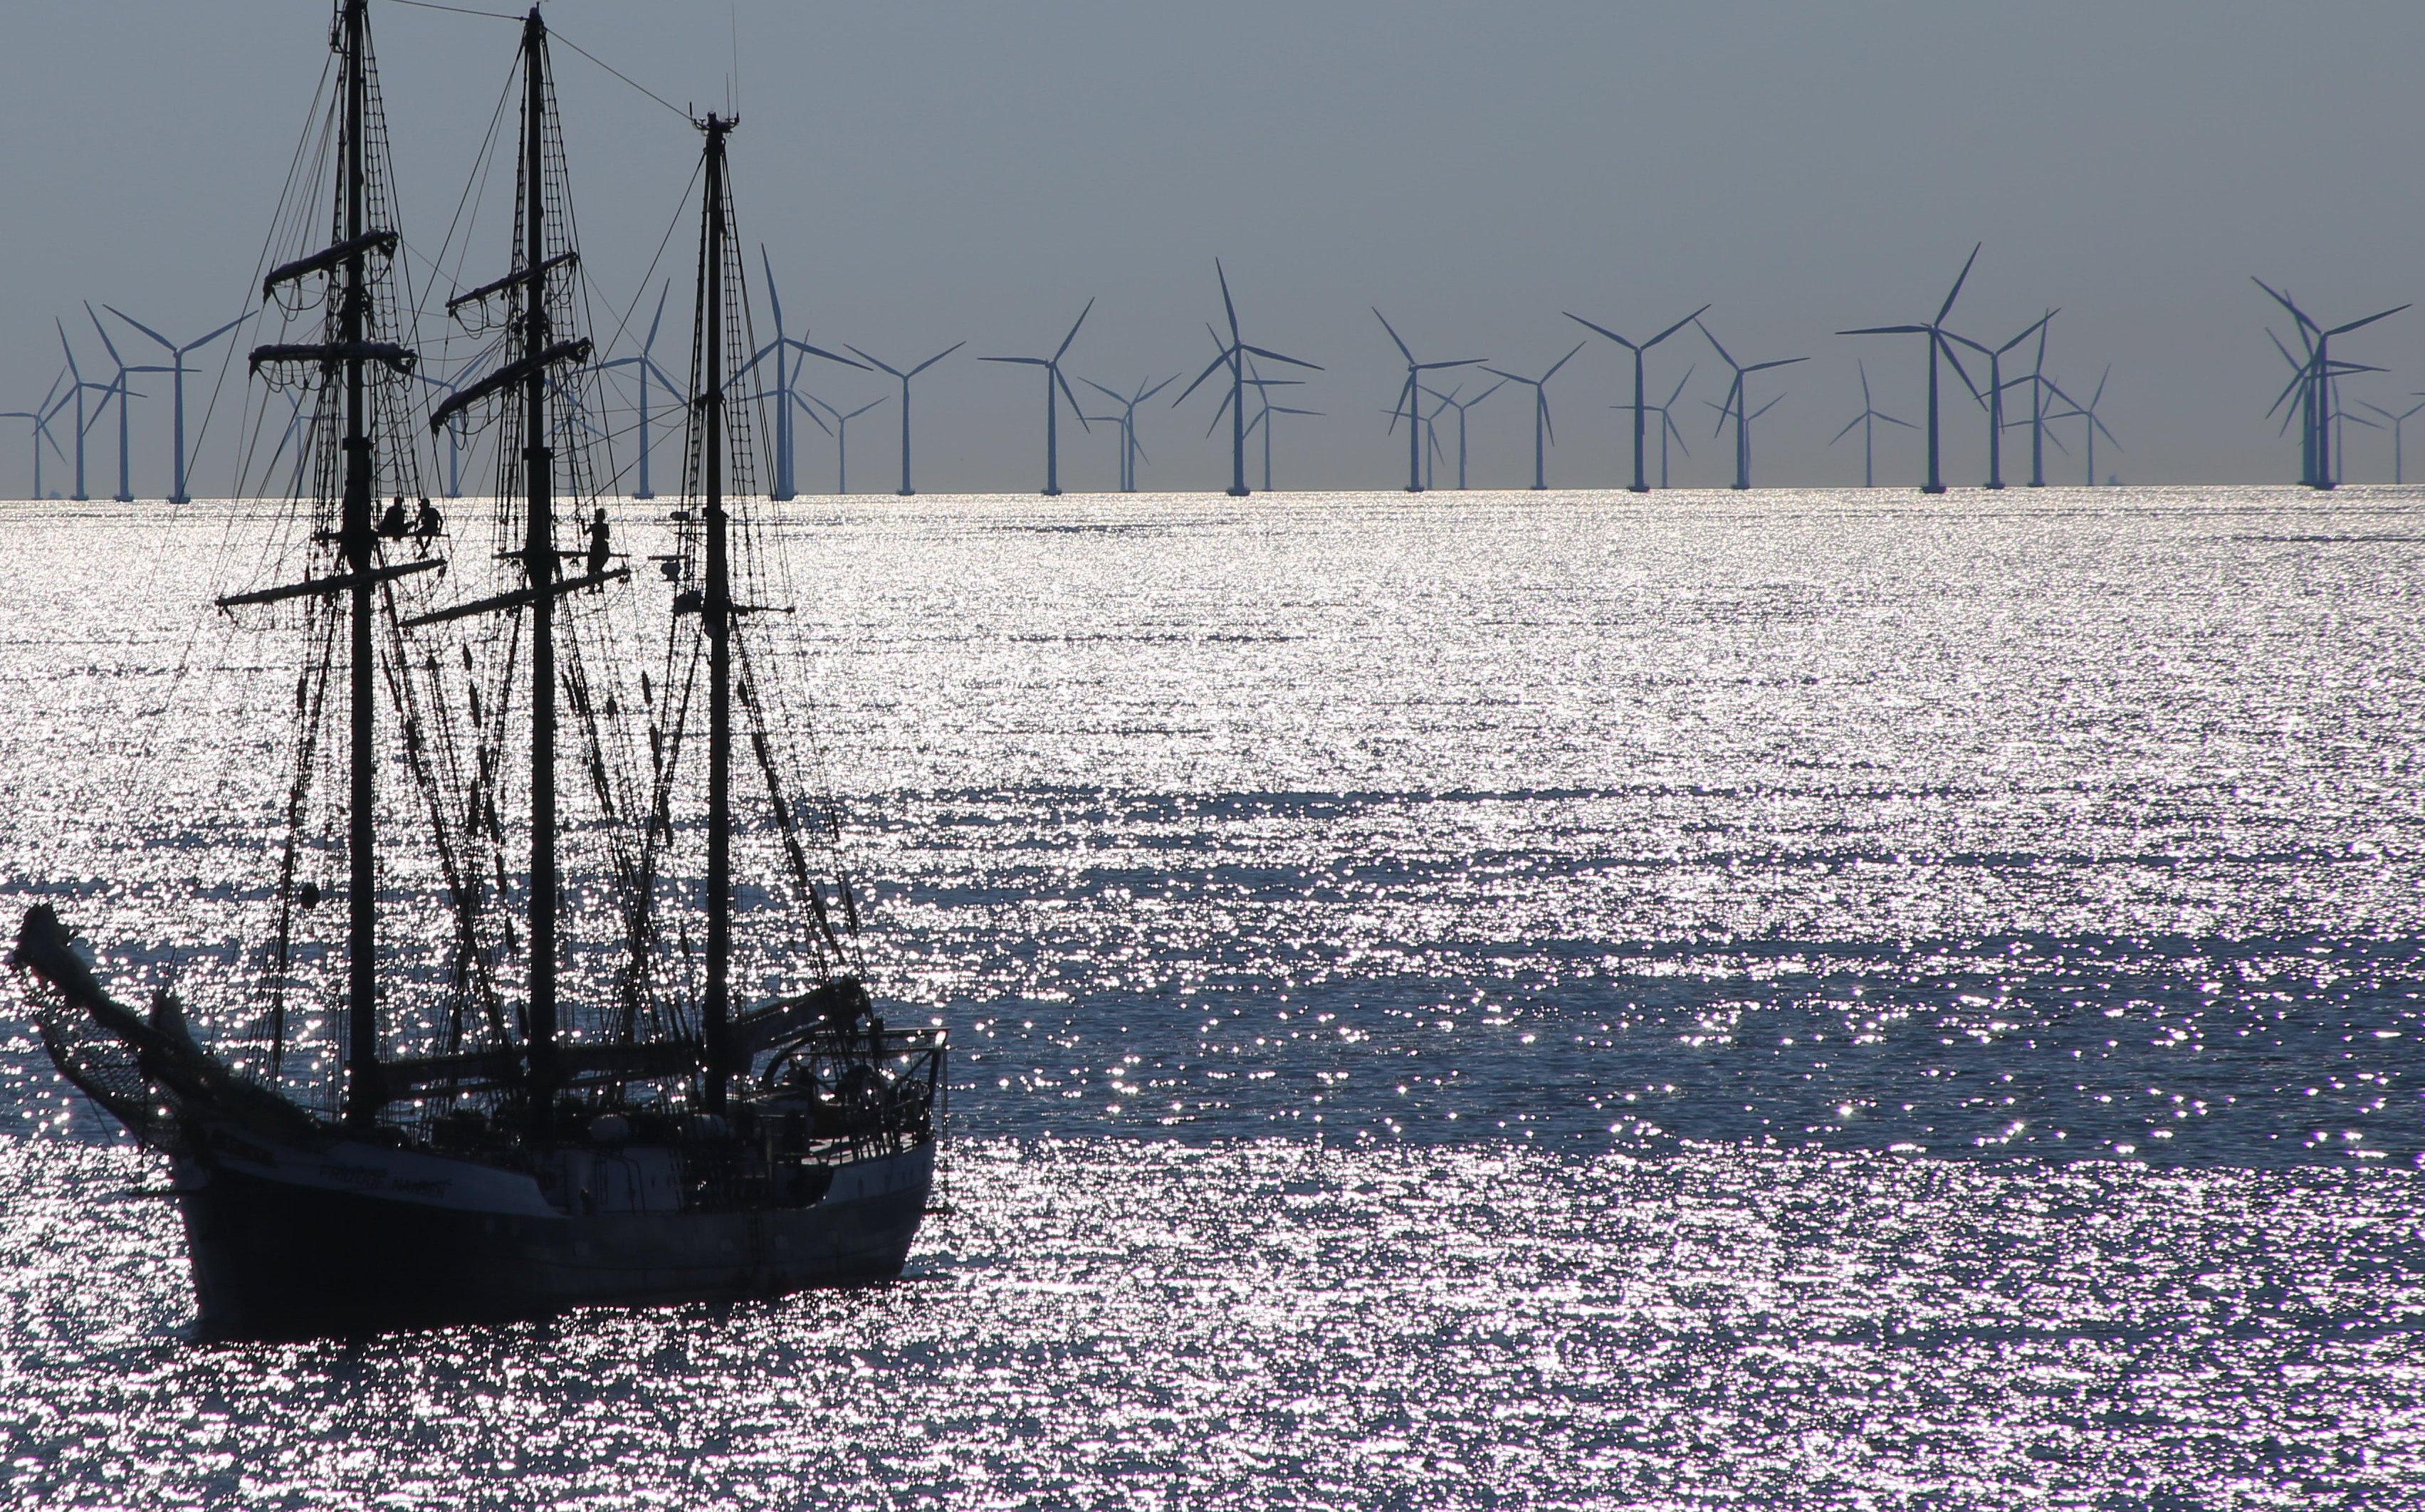
\includegraphics[height=\paperheight]{logos/photo_offshore.jpg}}

\usetheme[background=light,sectionstyle=style2]{trigon}

% Define logos to use (comment if no logo)
%\biglogo{trigon_full.pdf} % Used on titlepage only
%\smalllogo{trigon_small.pdf} % Used on top right corner of regular frames

\biglogo{logos/uliege_uliege.pdf} % Used on titlepage only
\smalllogo{logos/uliege_small.pdf} % Used on top right corner of regular frames


% ------ If you want to change the theme default colors, do it here ------
%\definecolor{tTheme}{HTML}{00843B}   % Green
%\definecolor{tPrim}{HTML}{00843B}   % Green
%\definecolor{tSec}{HTML}{289B38}    % Green light
%\definecolor{tAccent}{HTML}{F07F3C} % Orange


% ------ Packages and definitions used for this demo. Can be removed ------
\usepackage{appendixnumberbeamer} % To use \appendix command
\pdfstringdefDisableCommands{% Fix hyperref translate warning with \appendix
  \def\translate#1{#1}%
}
\usepackage{pgf-pie} % For pie charts
\usepackage{caption} % For subfigures
\usepackage{subcaption} % For subfigures
\usepackage{xspace}
\newcommand{\themename}{\textbf{\textsc{trigon}}\xspace}
\usepackage[scale=2]{ccicons} % Icons for CC-BY-SA
\usepackage{booktabs} % Better tables
%sqaddded
\graphicspath{ {./images/} }
\usepackage{eurosym}
\usepackage{makecell} 
\usepackage{tikz}
\usetikzlibrary{shapes.geometric, arrows.meta, positioning, decorations.pathreplacing, calc}
\setbeamerfont{frametitle}{size=\Large} 


%==============================================================================
%                               BEGIN DOCUMENT
%==============================================================================

\begin{document}

%--------------------------------------
% Create title frame
\titleframe





%==============================================
\section{Introduction}
%==============================================

\begin{frame}{\insertsectionhead}
  \frametitle{Introduction}
  %\framesubtitle{VRE capacity is rapidly expanding worldwide}
  \begin{figure}
    \centering
    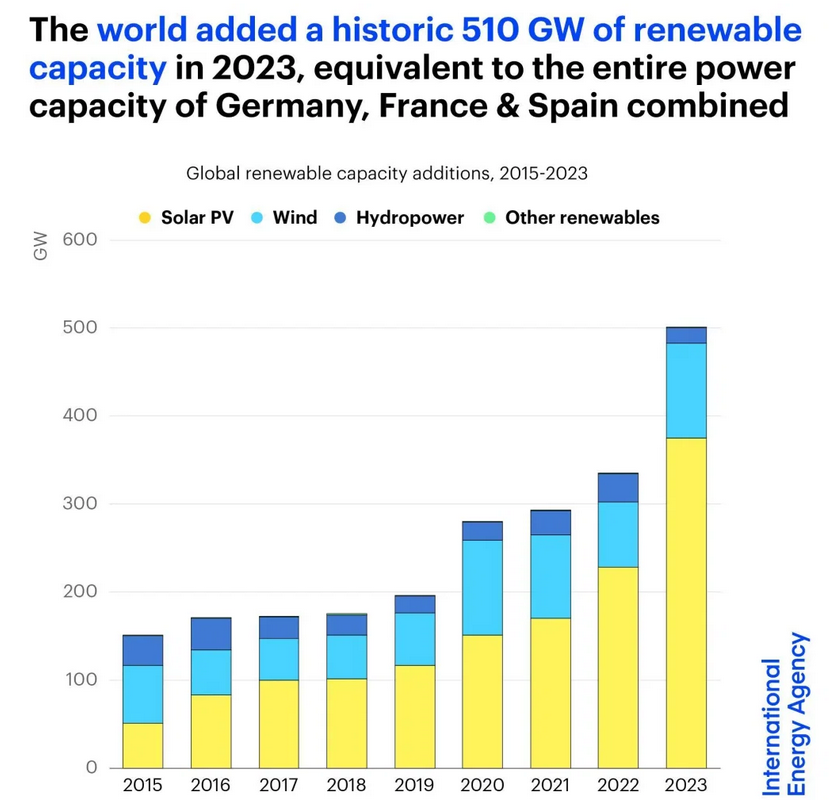
\includegraphics[width=0.5\textwidth]{global.png}
  \end{figure}
\end{frame}

\setbeamertemplate{frame footer}{\parbox[c][2.5ex][c]{\dimexpr\textwidth-5em\relax}{\centering\vspace*{0mm}\tiny Courtesy: Elia Dashboard\hfill}}
\begin{frame}
  \frametitle{Introduction}
  \framesubtitle{Characteristics of VRE technologies! Uncertainty and Variability}
  \begin{figure}
    \centering
    \begin{subfigure}[b]{0.49\textwidth}
      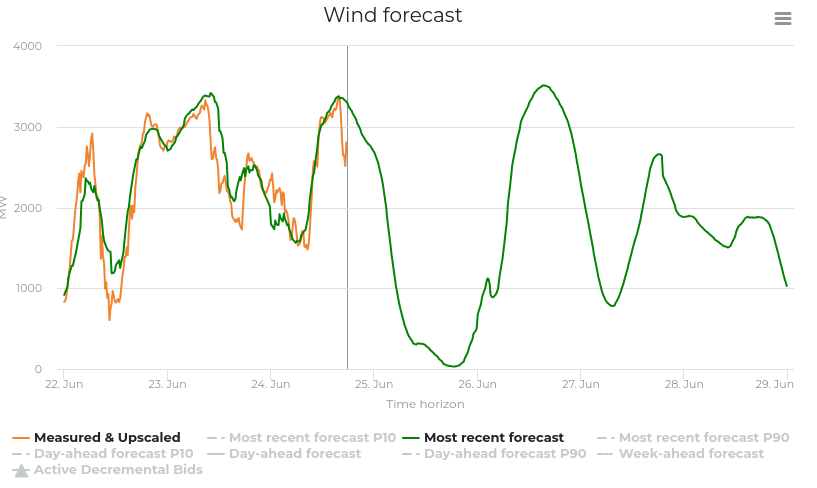
\includegraphics[width=\textwidth]{wind.png}
      \label{fig:s5s164}
    \end{subfigure}
    \hfill % space between images
    \begin{subfigure}[b]{0.49\textwidth}
      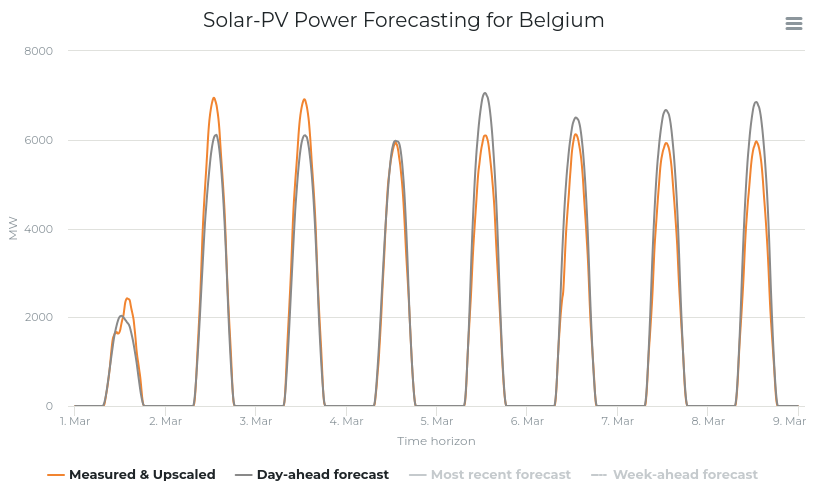
\includegraphics[width=\textwidth]{solar.png}
      \label{fig:s5s165}
    \end{subfigure}
    \caption*{\small A perfect forecast eliminates uncertainty, but variability remains}
  \end{figure}
  
\end{frame}

\setbeamertemplate{frame footer}{\parbox[c][2.5ex][c]{\dimexpr\textwidth-5em\relax}{\centering\vspace*{0mm}\tiny Addapted from Ueckerdt et al. 2013\hfill}}
\begin{frame}
  \frametitle{Introduction}
  \framesubtitle{Integration costs: the additional system cost
when integrating VRE}
  \begin{figure}
    \centering
    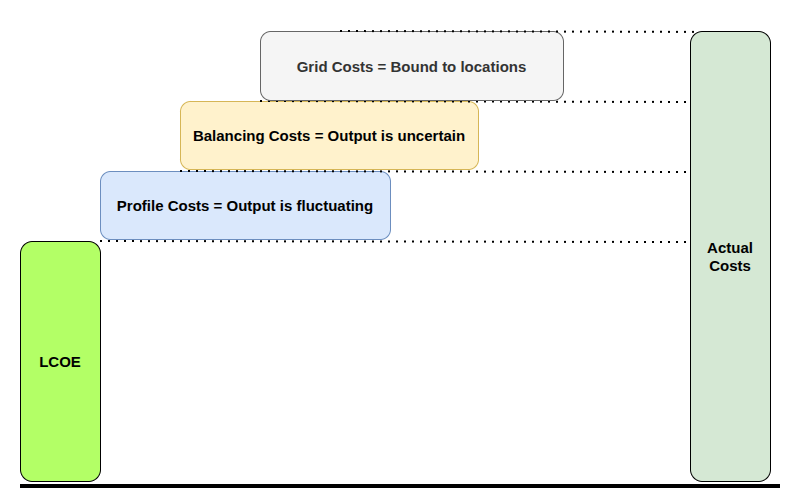
\includegraphics[width=0.7\textwidth]{prof.png}
  \end{figure}
\end{frame}


\setbeamertemplate{frame footer}{} % Clear footer for next slides
\begin{frame}
\frametitle{Introduction}
\framesubtitle{Methodologies used to compute integration costs (literature review)}
  \begin{figure}
    \centering
    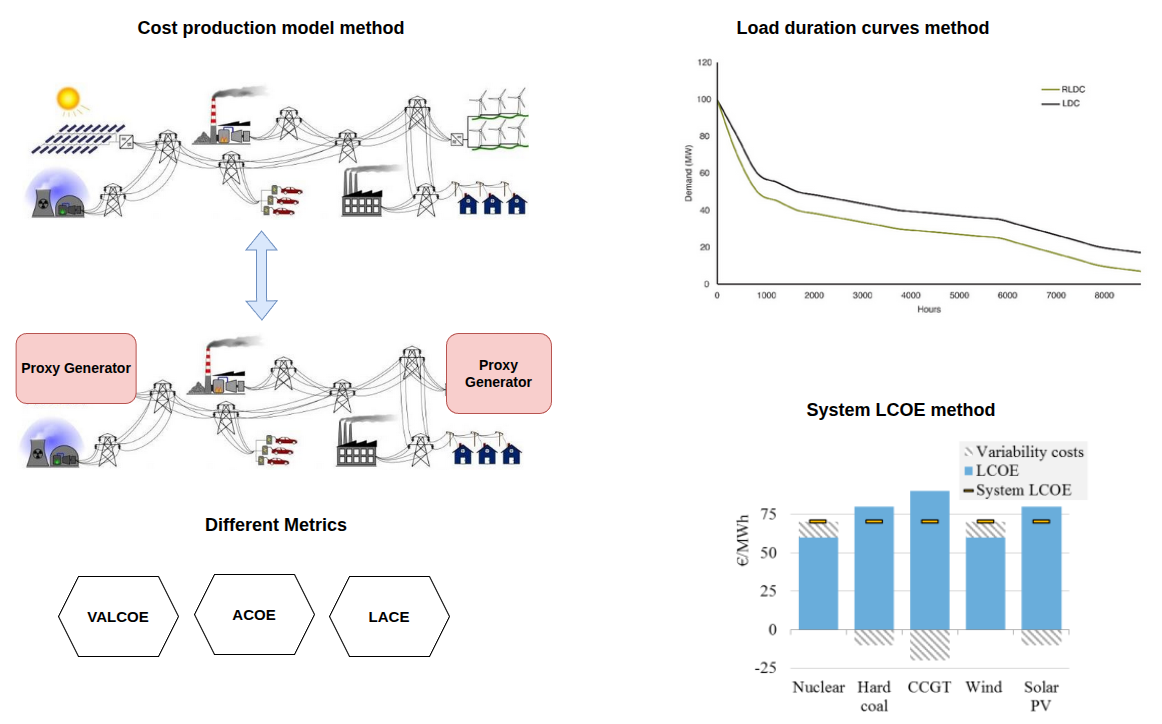
\includegraphics[width=0.7\textwidth]{mehod.png}
  \end{figure}
\end{frame}

%==============================================
\section{Methodology}
%==============================================

\begin{frame}
  \centering
  \Large \textbf{Objective} \par
  \vspace{0.5em}
  \Large Compute the integration costs in a simple and straightforward way! \par
  \vspace{1em}
  \Large {Utilize an energy system model}
\end{frame}

\setbeamertemplate{frame footer}{\parbox[c][2.5ex][c]{\dimexpr\textwidth-5em\relax}{\centering\vspace*{1mm}\tiny Image credentials: PyPSA-Eur\hfill}}
\begin{frame}[fragile]
  \frametitle{Why PyPSA-Eur?}
  \begin{figure}
    \centering
    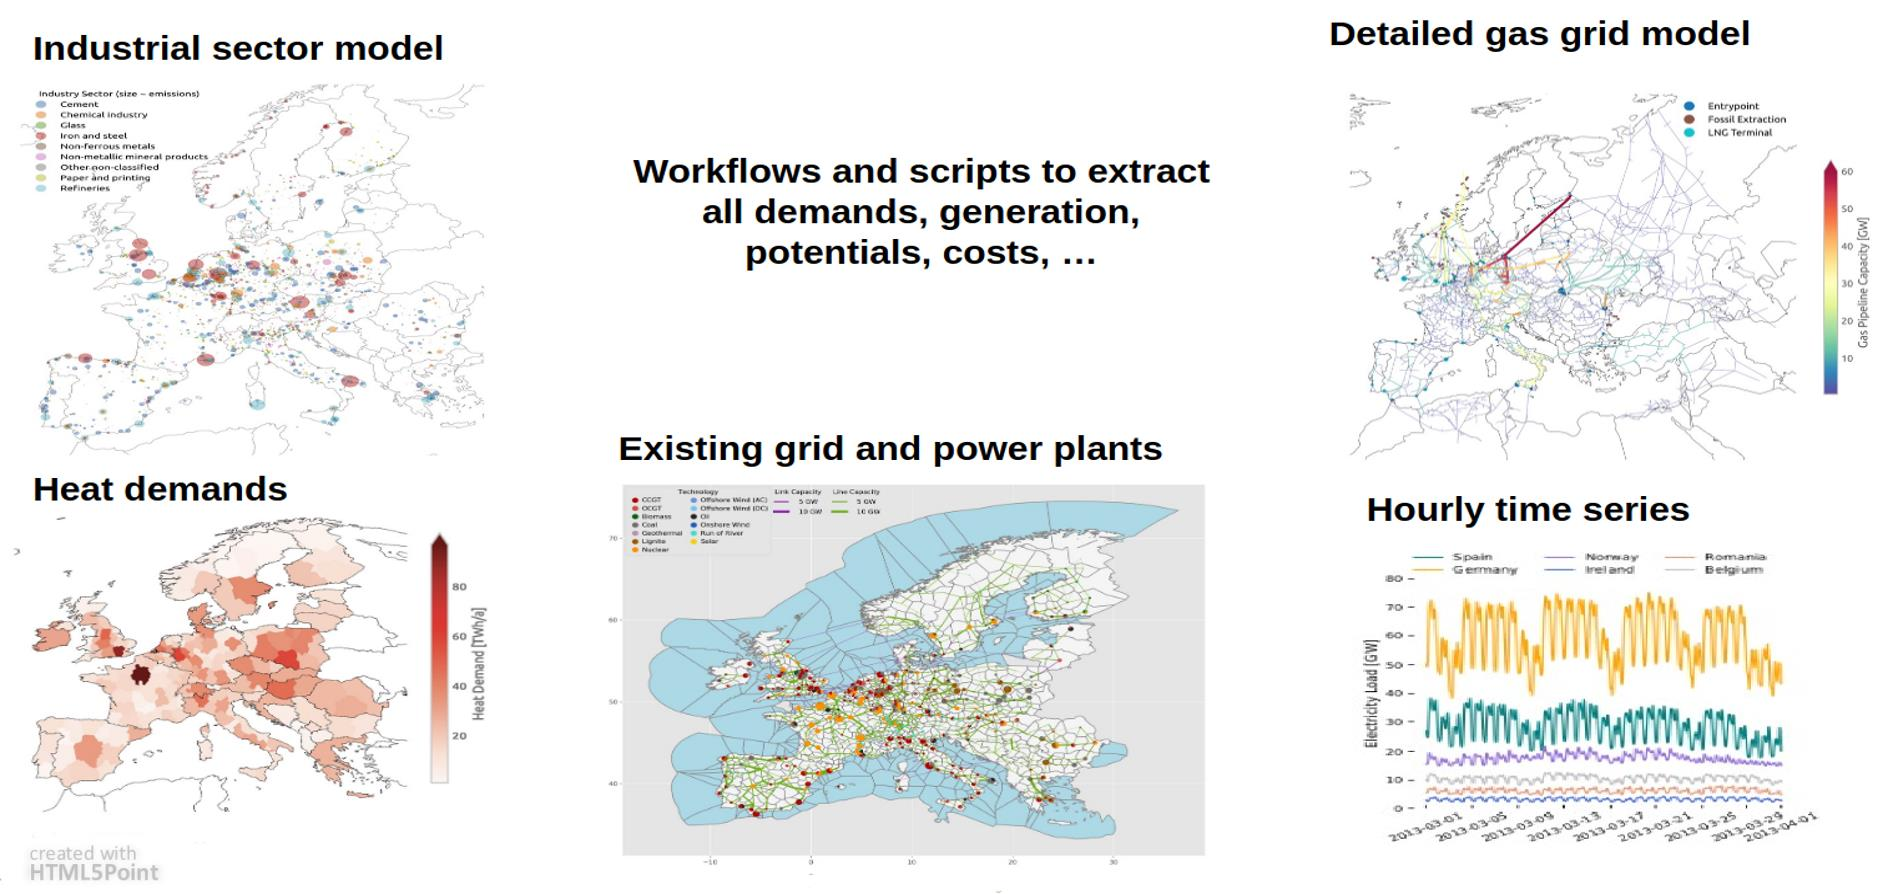
\includegraphics[width=0.9\textwidth]{s12s186.jpg}
  \end{figure}
\end{frame}

\setbeamertemplate{frame footer}{\parbox[c][2.5ex][c]{\dimexpr\textwidth-5em\relax}{\centering\vspace*{1mm}\tiny Image credentials: PyPSA-Eur\hfill}}
\begin{frame}{\insertsectionhead}

\begin{figure}
    \centering
    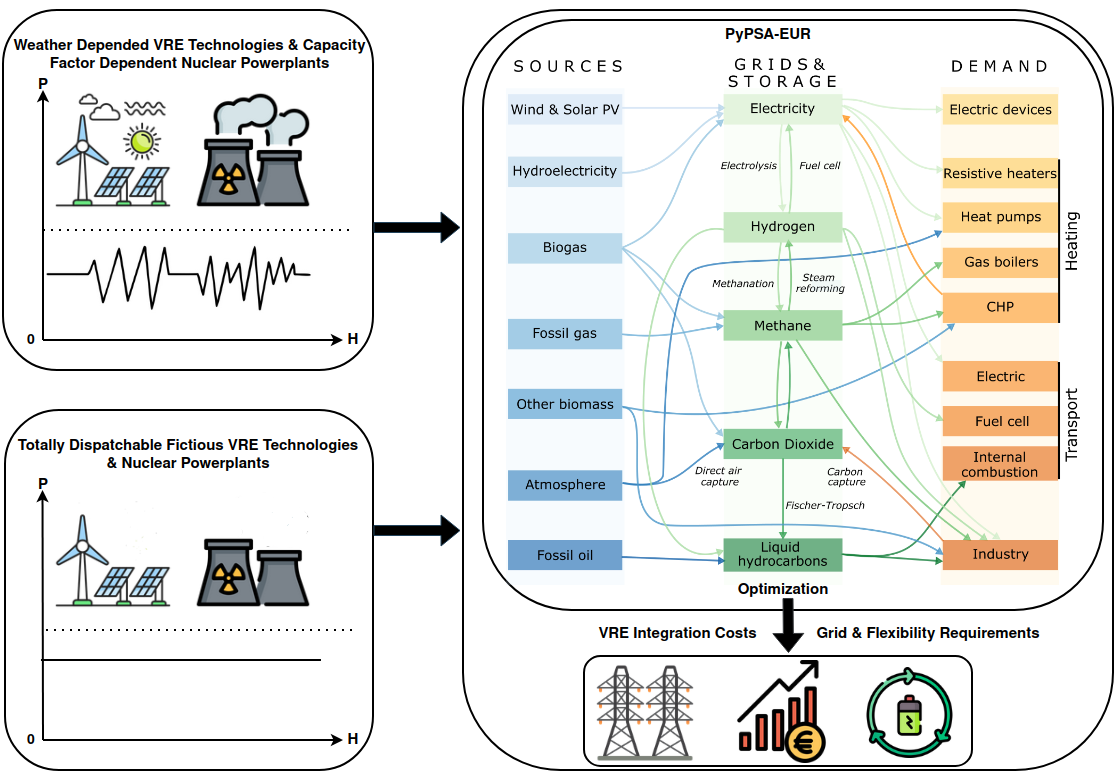
\includegraphics[width=0.65\textwidth]{method.png}
  \end{figure}
\end{frame}

\setbeamertemplate{frame footer}{} % Clear footer for next slides
\begin{frame}{\insertsectionhead}
\framesubtitle{ Reference scenario computes the total annualised system costs and optimised capacities of renewable technologies}
\begin{figure}
    \centering
    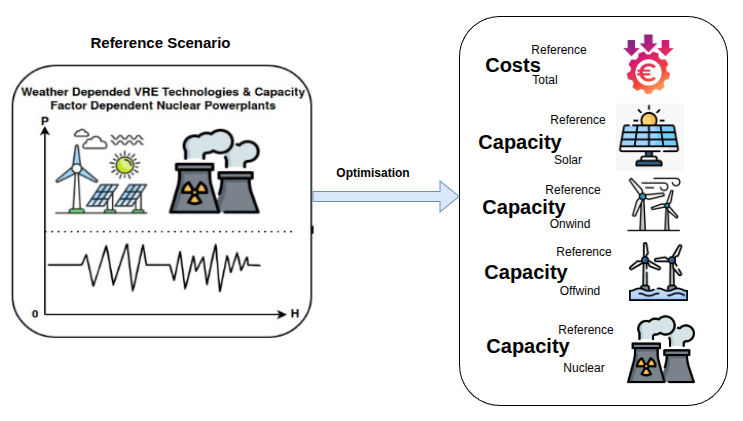
\includegraphics[width=0.7\textwidth]{method1.png}
  
  %\caption*{\small Reference scenario computes the total annualised system costs and optimised capacities of renewable technologies}
  \end{figure}
\end{frame}

\setbeamertemplate{frame footer}{} % Clear footer for next slides
\begin{frame}{\insertsectionhead}
\framesubtitle{Example: Solar Scenario}
\begin{figure}
    \centering
    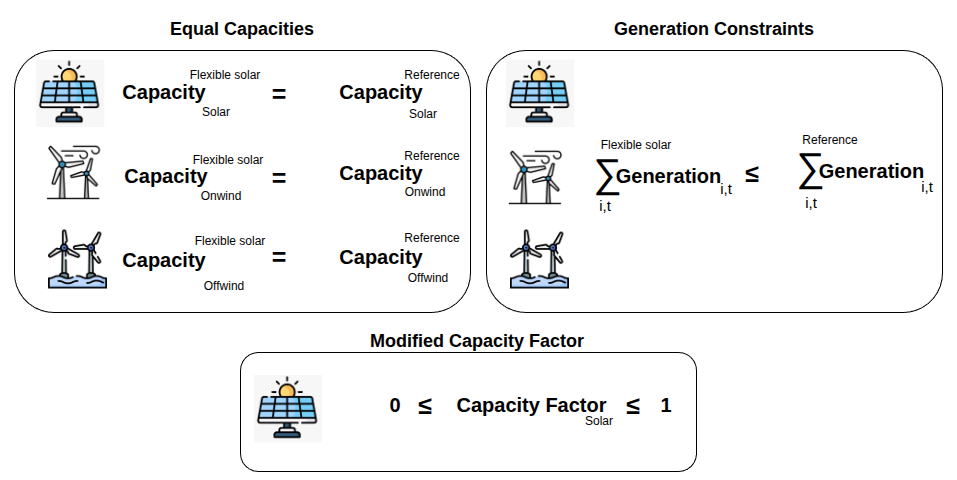
\includegraphics[width=0.9\textwidth]{cons.png}
  
  %\caption*{\small Reference scenario computes the total annualised system costs and optimised capacities of renewable technologies}
  \end{figure}
\end{frame}

\setbeamertemplate{frame footer}{} % Clear footer for next slides
\begin{frame}{\insertsectionhead}
\framesubtitle{Example: Solar Scenario}
\begin{figure}
    \centering
    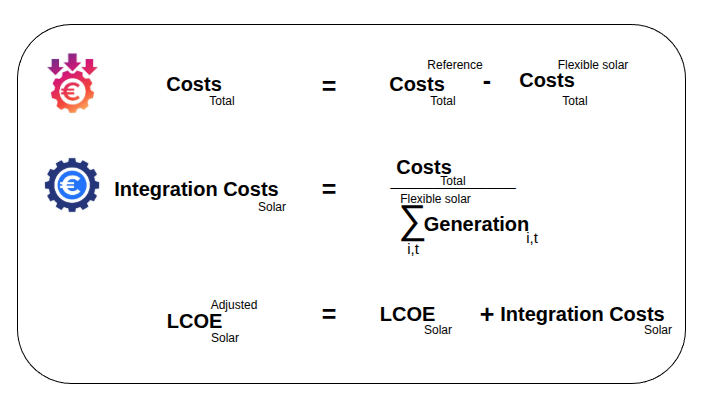
\includegraphics[width=0.7\textwidth]{metr.png}
  
  \caption*{\small Straight forward computation of integration costs}
  \end{figure}
\end{frame}
% End of section Energy Sufficiency
%----------------------------------------------------------------------------------------
% SLIDE 8
%----------------------------------------------------------------------------------------

\section{Scenarios}
%----------------------------------------------------------------------------------------
% SLIDE 9
%----------------------------------------------------------------------------------------
\begin{frame}[fragile]
  \frametitle{Scenarios}

  \textbf{5 Scenarios:} Solar, Onshore Wind, Offshore Wind, VRE, Nuclear \\
  \textbf{Considered Nodes:} BE, FR, NL, GB, DE \\
  
  \textbf{Optimisation:} Greenfield and brownfield

  \vspace{1em} % Adds vertical space

  \begin{columns}
    \begin{column}{0.5\textwidth}
      \textbf{Configuration:}
      \begin{itemize}
         \item \makebox[\linewidth][l]{Carbon budget: 2030 (–55\%), 2040 (–85\%), 2050 (net zero)}
        \item \makebox[\linewidth][l]{Current demand projections + expected efficiency improvements}
        \item \makebox[\linewidth][l]{Transmission lines espansion, 50\% in each planning horizon}
        \item \makebox[\linewidth][l]{Increased EV shares upto 85\% by 2050}
        \item CCS is allowed
      \end{itemize}
    \end{column}

    \begin{column}{0.5\textwidth}
      % Optional: add another scenario or info here
    \end{column}
  \end{columns}
\end{frame}



%==============================================
\section{Results}
%==============================================
\begin{frame}{\insertsectionhead}
\framesubtitle{Integration costs in all scenarios}
\begin{figure}
    \centering
    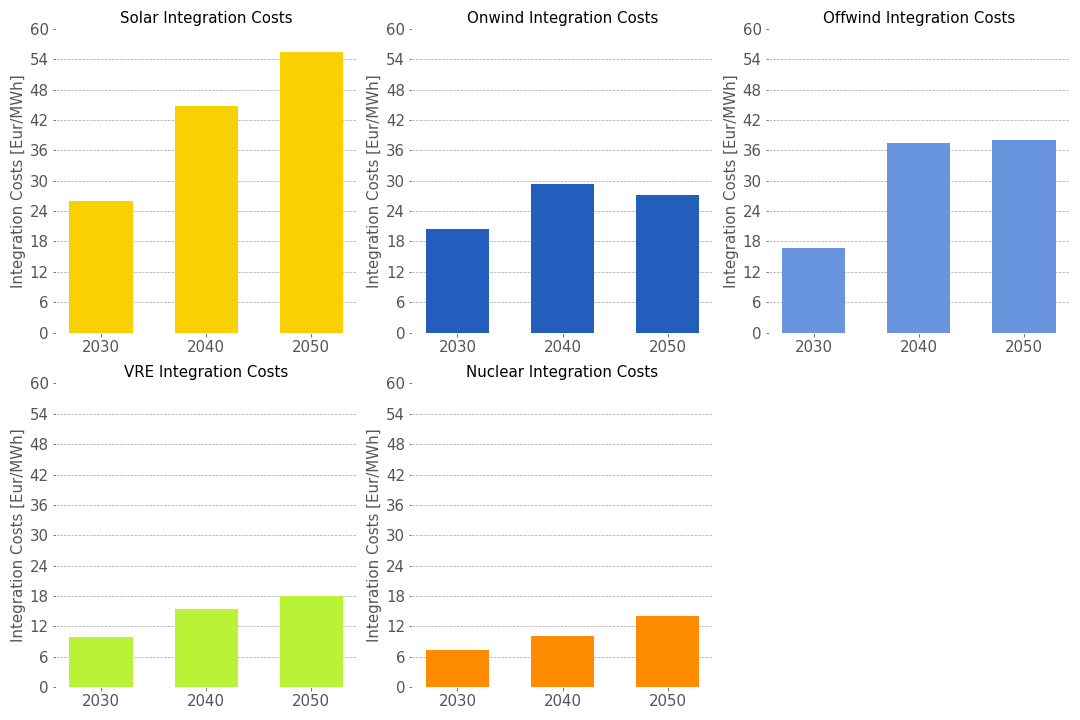
\includegraphics[width=0.65\textwidth]{overnight_inti.png}
  
  \end{figure}
\end{frame}

\begin{frame}{\insertsectionhead}
\framesubtitle{Integration costs with penetration level in power system}
\begin{figure}
    \centering
    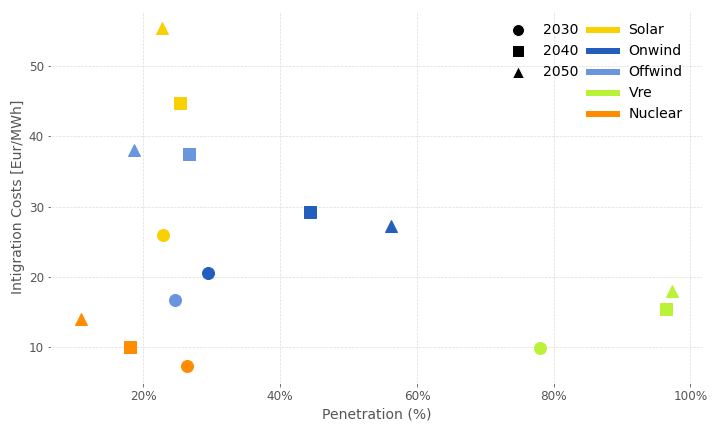
\includegraphics[width=0.7\textwidth]{pen.png}
  
  \end{figure}
\end{frame}


\begin{frame}{\insertsectionhead}
\framesubtitle{Distribution of integration costs}
\begin{figure}
    \centering
    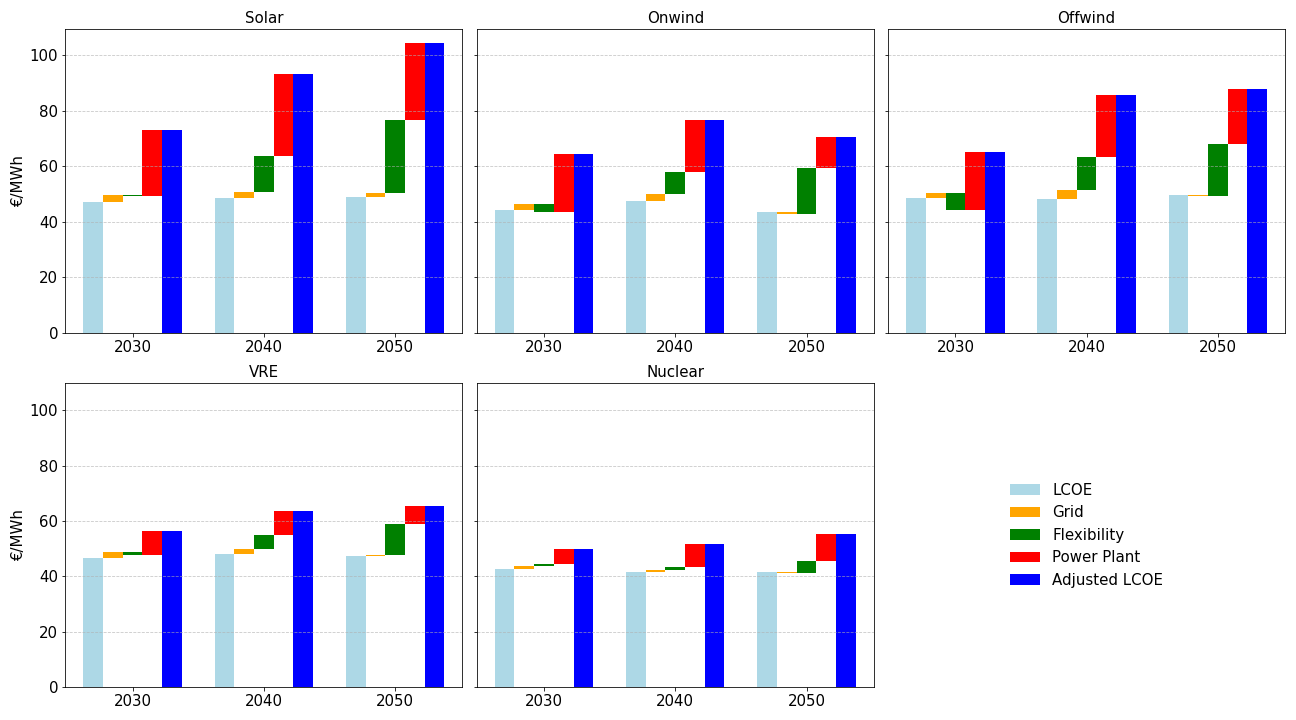
\includegraphics[width=0.85\textwidth]{cossts.png}
  
  \end{figure}
\end{frame}

\begin{frame}{\insertsectionhead}
\frametitle{IEA- VALCOE}
\begin{figure}
    \centering
    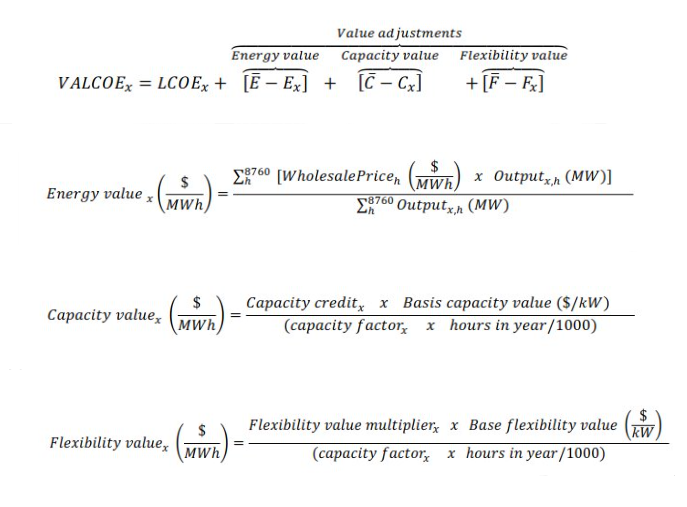
\includegraphics[width=0.6\textwidth]{valcoe.png}
  
  \end{figure}
\end{frame}

\begin{frame}{\insertsectionhead}
\framesubtitle{Comaprison with VALCOE}
\begin{figure}
    \centering
    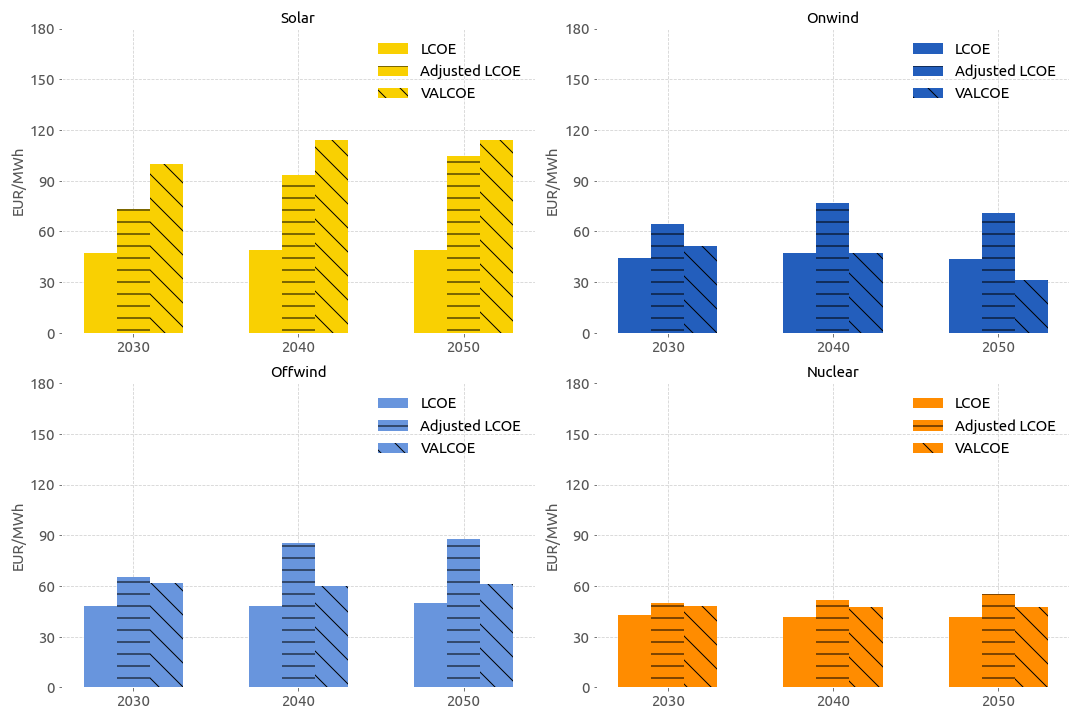
\includegraphics[width=0.6\textwidth]{valcoe_over.png}
  
  \end{figure}
\end{frame}
%==============================================
\section{Conclusions}
%==============================================

% SLIDE 19
\begin{frame}[fragile]
  \frametitle{Conclusion and Future Work}

  \textbf{Conclusion:}
    \begin{itemize}
      \item {Integration costs computations can be made in a simple way using existing modeling tools.}
      \item {Individually, these costs can be very high for some VRE technologies like solar.}
      \item {Policy measures have a big impact on VRE integration; when combined, integration costs remain marginal even above 80\% penetration.}
    \end{itemize}

  \textbf{Future Work:}
    \begin{itemize}
      \item Extending the study on regional level.
      \item Considering the operational constraints of powerplants.
       \item Comparison of results with other studies.
      \item Sensitivity analysis.
      
    \end{itemize}
\end{frame}




\section{Thank You!}



\end{document}